\documentclass[preprint, 3p,
authoryear]{elsarticle} %review=doublespace preprint=single 5p=2 column
%%% Begin My package additions %%%%%%%%%%%%%%%%%%%

\usepackage[hyphens]{url}

  \journal{An Awesome Journal} % Sets Journal name

\usepackage{graphicx}
%%%%%%%%%%%%%%%% end my additions to header

\usepackage[T1]{fontenc}
\usepackage{lmodern}
\usepackage{amssymb,amsmath}
% TODO: Currently lineno needs to be loaded after amsmath because of conflict
% https://github.com/latex-lineno/lineno/issues/5
\usepackage{lineno} % add
\usepackage{ifxetex,ifluatex}
\usepackage{fixltx2e} % provides \textsubscript
% use upquote if available, for straight quotes in verbatim environments
\IfFileExists{upquote.sty}{\usepackage{upquote}}{}
\ifnum 0\ifxetex 1\fi\ifluatex 1\fi=0 % if pdftex
  \usepackage[utf8]{inputenc}
\else % if luatex or xelatex
  \usepackage{fontspec}
  \ifxetex
    \usepackage{xltxtra,xunicode}
  \fi
  \defaultfontfeatures{Mapping=tex-text,Scale=MatchLowercase}
  \newcommand{\euro}{€}
\fi
% use microtype if available
\IfFileExists{microtype.sty}{\usepackage{microtype}}{}
\usepackage[]{natbib}
\bibliographystyle{elsarticle-harv}

\ifxetex
  \usepackage[setpagesize=false, % page size defined by xetex
              unicode=false, % unicode breaks when used with xetex
              xetex]{hyperref}
\else
  \usepackage[unicode=true]{hyperref}
\fi
\hypersetup{breaklinks=true,
            bookmarks=true,
            pdfauthor={},
            pdftitle={Cost-Effectiveness of Biomarker-Driven First-Line Immunotherapy in Advanced Melanoma: A Mathematical Modeling Approach},
            colorlinks=false,
            urlcolor=blue,
            linkcolor=magenta,
            pdfborder={0 0 0}}

\setcounter{secnumdepth}{5}
% Pandoc toggle for numbering sections (defaults to be off)


% tightlist command for lists without linebreak
\providecommand{\tightlist}{%
  \setlength{\itemsep}{0pt}\setlength{\parskip}{0pt}}




\usepackage{booktabs}
\usepackage{graphicx}
\usepackage{threeparttable}
\usepackage{float}
\usepackage{caption}
\usepackage{tabularx}
\usepackage{longtable}



\begin{document}


\begin{frontmatter}

  \title{Cost-Effectiveness of Biomarker-Driven First-Line Immunotherapy
in Advanced Melanoma: A Mathematical Modeling Approach}
    \author[Harvard University]{Jacob Jameson%
  \corref{cor1}%
  \fnref{1}}
   \ead{jacobjameson@g.harvard.edu} 
    \author[Harvard University]{Soroush Saghafian%
  %
  \fnref{1}}
  
    \author[Dana Farber Cancer Institute]{Giuseppe Tarantino%
  %
  \fnref{2}}
  
    \author[Dana Farber Cancer Institute]{David Liu%
  %
  \fnref{2}}
  
      \affiliation[Some Institute of Technology]{
    organization={Big Wig University},addressline={1 Main
Street},city={Gotham},postcode={123456},state={State},country={United
States},}
    \affiliation[Another University]{
    organization={Department},addressline={A Street
29},city={Manchester},postcode={2054 NX},country={The Netherlands},}
    \cortext[cor1]{Corresponding author}
    \fntext[1]{This is the first author footnote.}
    \fntext[2]{Another author footnote.}
  
  \begin{abstract}
  \textbf{Background:} Immune checkpoint inhibitors (ICIs) have
  dramatically improved the prognosis of advanced melanoma, yet
  substantial heterogeneity in response and toxicity persists. Recent
  work by Tarantino et al.~has shown that genomic heterogeneity and
  ploidy robustly predict intrinsic resistance to PD-1 blockade. We
  propose a simulation model to compare the cost-effectiveness of
  standard first-line treatment strategies versus a biomarker-based
  strategy that leverages genomic predictors.

  \textbf{Methods:} We reconstructed individual patient data (IPD) from
  the published Kaplan--Meier curves of the CheckMate 067 trial and
  fitted parametric and spline survival models to derive monthly
  transition probabilities. A discrete-time Markov model---with three
  health states (stable disease, progressive disease, and death) and a
  1-month cycle over a 10-year horizon---was constructed to simulate
  costs, quality-adjusted life-years (QALYs), and toxic effects. In an
  extended analysis, we incorporated the predictive performance
  (sensitivity, specificity, and PPV) reported by Tarantino et al.~to
  simulate a biomarker-based treatment allocation strategy. Model
  inputs, including survival probabilities, utilities, and costs, were
  derived from published literature and calibrated against trial data.

  \textbf{Results:} {[}Insert calibrated model results,
  cost-effectiveness outcomes, and sensitivity analyses here.{]}

  \textbf{Conclusions:} Our initial results indicate that a
  biomarker-driven treatment allocation strategy may be cost-effective
  compared with a standard one-size-fits-all approach for first-line
  immunotherapy in advanced melanoma. These findings underscore the
  potential for personalized treatment strategies to improve clinical
  outcomes and resource utilization.
  \end{abstract}
    \begin{keyword}
    cost-effectiveness \sep immunotherapy \sep melanoma \sep biomarker \sep 
    mathematical model
  \end{keyword}
  
 \end{frontmatter}

\section{Introduction}\label{introduction}

Immune checkpoint inhibitors (ICIs) have revolutionized the treatment of
advanced melanoma, leading to unprecedented long-term survival in a
subset of patients. The CheckMate 067 trial demonstrated that both
nivolumab monotherapy and the combination of nivolumab with ipilimumab
offer superior overall survival (OS) and progression-free survival (PFS)
compared with ipilimumab monotherapy. However, significant toxicities
associated with combination therapy and the heterogeneous treatment
response across patients necessitate a more personalized approach.

Recent work by Tarantino et al.~has shown that genomic heterogeneity and
ploidy can robustly predict intrinsic resistance to PD-1 blockade. These
findings provide a basis for a biomarker-driven treatment strategy
whereby patients predicted to be intrinsically resistant to single-agent
PD-1 blockade may preferentially receive combination immunotherapy. In
this study, we propose a simulation model to evaluate the
cost-effectiveness of standard first-line treatment strategies versus a
biomarker-based strategy that leverages genomic predictors.

Our objectives are to: - Calibrate a Markov model using reconstructed
individual patient data from the CheckMate 067 trial. - Estimate monthly
transition probabilities for OS and PFS based on parametric and spline
survival models. - Compare the cost-effectiveness of nivolumab
monotherapy and combination nivolumab plus ipilimumab. - Extend the
model by incorporating the predictive performance of the genomic
biomarker from Tarantino et al.~to simulate a biomarker-based treatment
allocation strategy.

\section{Methods}\label{methods}

\subsection{Decision Model}\label{decision-model}

We compared the cost-effectiveness of a biomarker-driven treatment
allocation strategy versus a standard one-size-fits-all approach for
first-line immunotherapy in advanced melanoma. The standard strategy
involved treating all patients with nivolumab monotherapy, while the
biomarker-driven strategy allocated patients to either nivolumab only or
nivolmab plus ipilimumab based on their predicted response to
single-agent PD-1 blockade. We created a Markov model to simulate
treatments, adverse events, quality of life, costs, and survival among
simulated patients. The state transition diagram (Figure
\hyperref[fig:model]{\ref{fig:model}}) shows how patients move through
the Markov model. The three main health states were stable disease,
cancer progression, and death. Our cost-effectiveness model used a
one-month cycle length extending over a 10-year time horizon, which is
the length of time for the final follow-up in the CheckMate 067 trial
\citep{checkmate067}. The Markov and survival models were constructed
and analyzed in R (version 4.4.2). The design and reporting of this
cost-effectiveness analysis follow standard guidelines published
elsewhere {[}\cite{Sanders2016}{]}.

\subsection{Model Structure}\label{model-structure}

We developed a discrete-time Markov model to simulate a cohort of
patients with advanced melanoma receiving first-line ICI. The model
includes three primary health states:

\begin{itemize}
\item
  \textbf{Stable Disease (Progression-Free):} Patients receiving
  treatment without disease progression.
\item
  \textbf{Progressive Disease:} Patients with disease progression.
\item
  \textbf{Death:} An absorbing state.
\end{itemize}

A one-month cycle length was used over a 10-year time horizon. Patients
may also experience treatment-related adverse events, which incur
additional costs and temporary utility decrements. The model was
implemented in R (version 4.0.2) using custom code and packages such as
\textbf{heemod} for cost-effectiveness analysis.

The evolution of the cohort is mathematically defined by the following
equations: \[
\begin{aligned}
S(t+1) &= S(t) \times (1 - p_{\text{prog}} - p_{\text{death}}), \\
P(t+1) &= S(t) \times p_{\text{prog}} + P(t) \times (1 - q_{\text{death}}), \\
D(t+1) &= D(t) + S(t) \times p_{\text{death}} + P(t) \times q_{\text{death}},
\end{aligned}
\] where:

\begin{itemize}
\item
  \(p_{\text{prog}}\) is the monthly probability of progression from the
  stable state,
\item
  \(p_{\text{death}}\) is the monthly probability of death from the
  stable state,
\item
  \(q_{\text{death}}\) is the monthly probability of death from the
  progressive state.
\end{itemize}

Figure \hyperref[fig:model]{\ref{fig:model}} displays the
state-transition diagram of the model.

\begin{figure}[h]
\centering
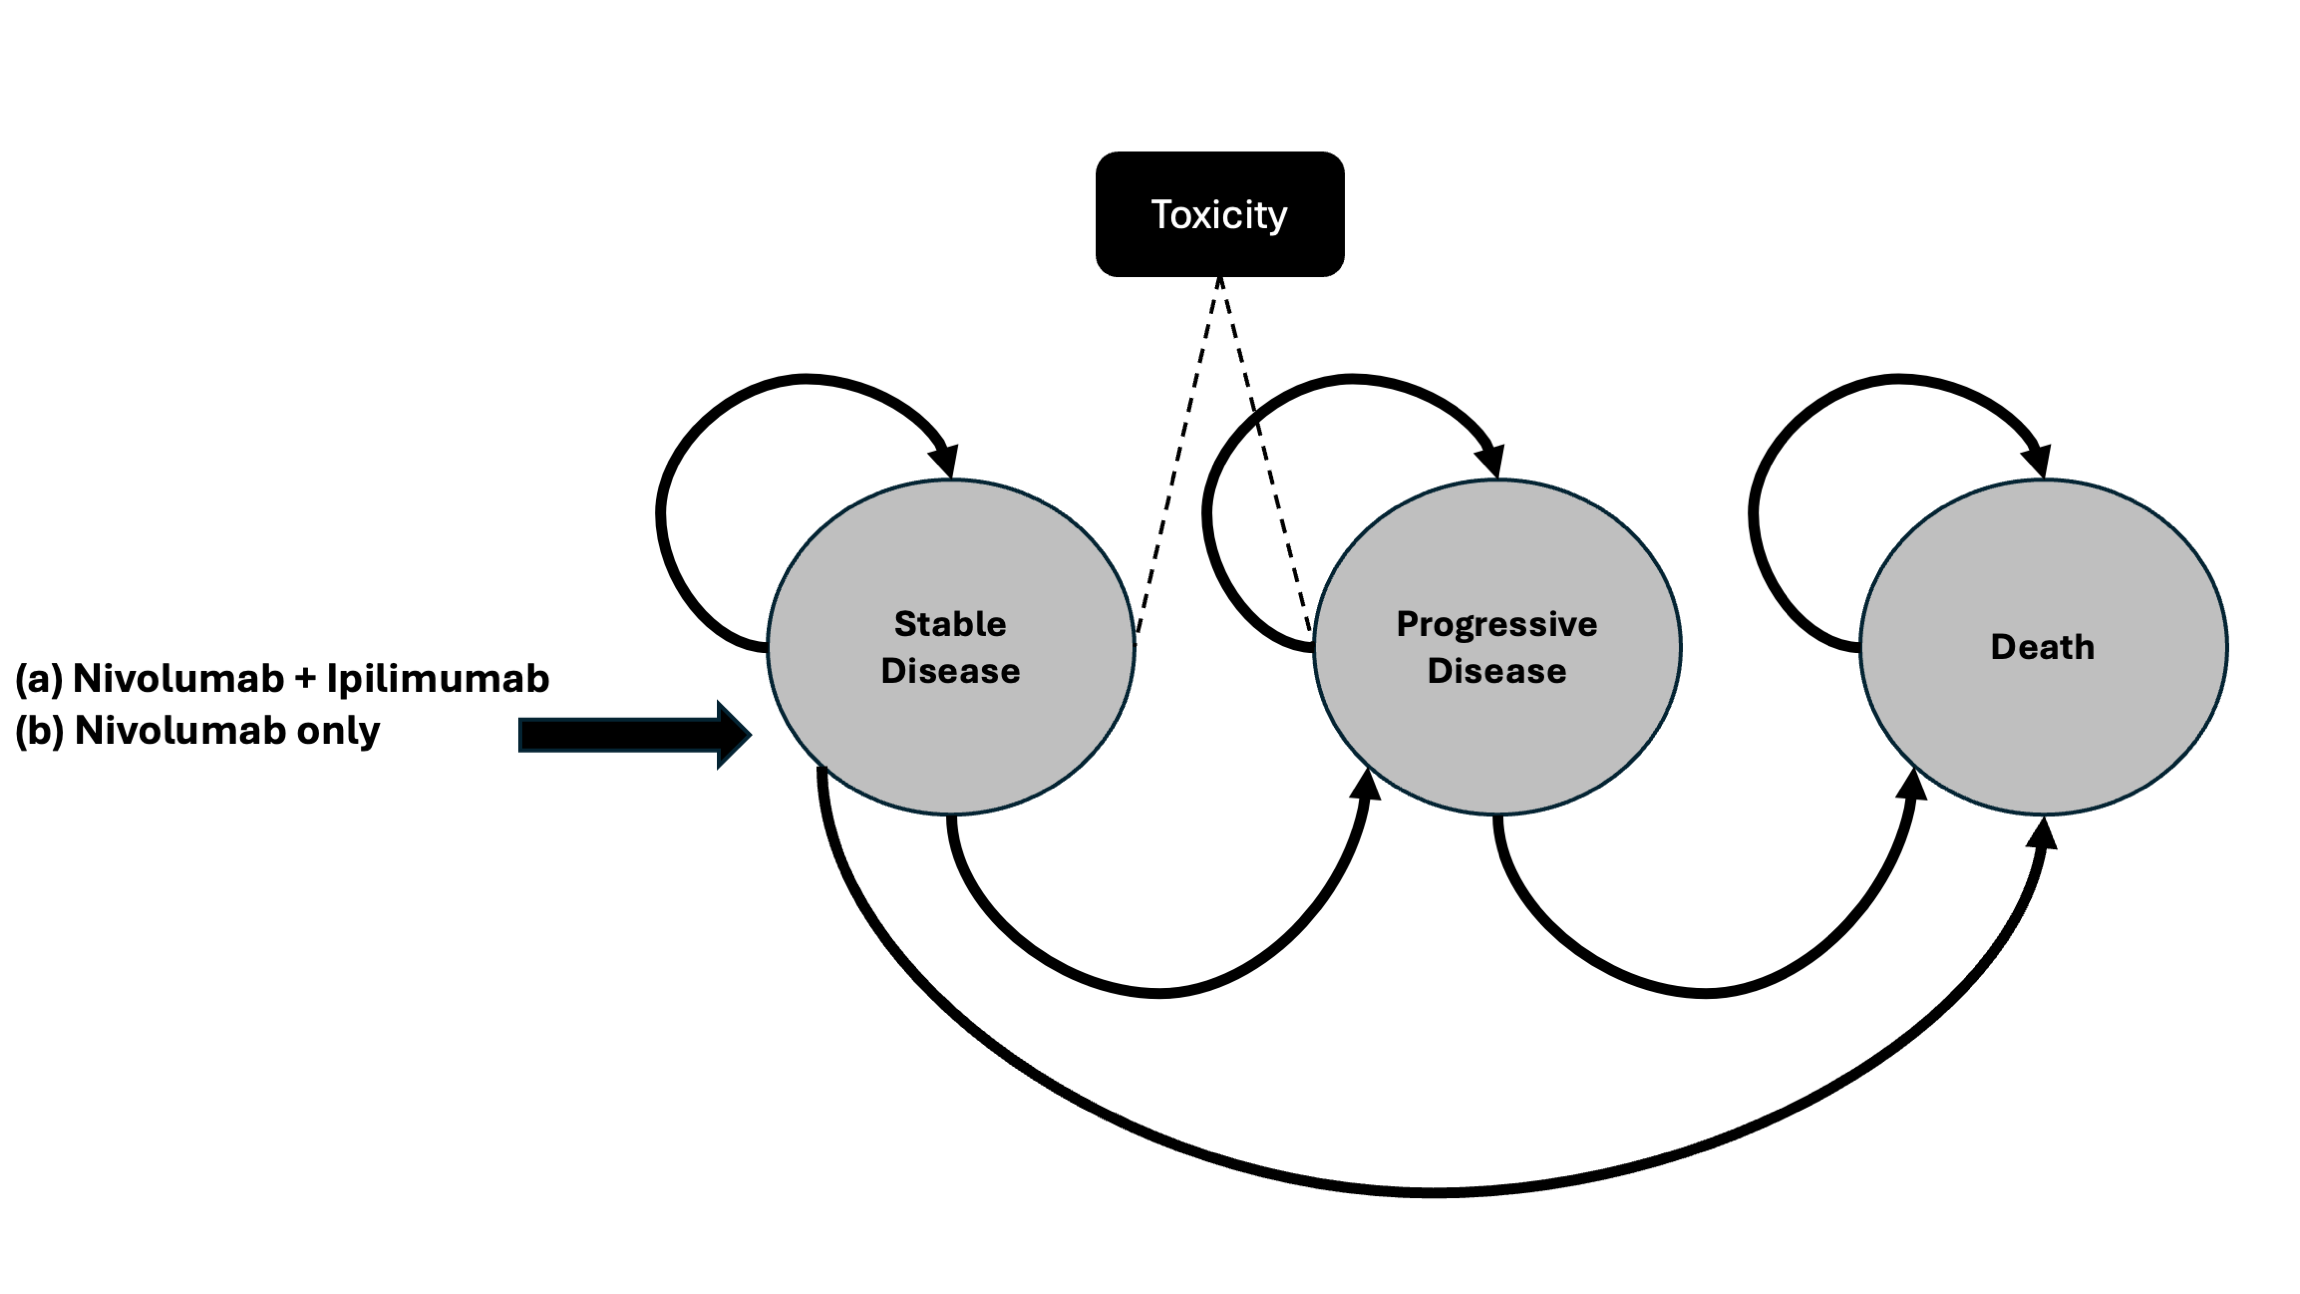
\includegraphics[width=\textwidth]{../outputs/model.png}
\caption{State-transition diagram of the Markov model. Patients transition between stable disease, progressive disease, and death. Adverse events are modeled as temporary events with associated cost and utility decrements.}
\label{fig:model}
\begin{tablenotes}
\footnotesize
\item \textit{Note}: Arrows indicate possible transitions. Patients experiencing toxicity remain in their current health state but incur additional costs and a reduction in utility.
\end{tablenotes}
\end{figure}

\subsection{Model Probabilities and
Calibration}\label{model-probabilities-and-calibration}

Transition probabilities for OS and PFS were estimated by reconstructing
individual patient data (IPD) from the published Kaplan--Meier curves in
CheckMate 067. We digitized the curves for both the nivolumab
monotherapy and the combination (nivolumab plus ipilimumab) arms using
GetData Graph Digitizer, then generated pseudo-IPD with the
\textbf{IPDfromKM} package in R. Parametric models (e.g., exponential,
Weibull, log-logistic) and natural cubic spline models were fitted to
the reconstructed data. The best-fitting models, selected based on the
Akaike information criterion (AIC), provided the monthly probabilities
of disease progression and death. Figure
\hyperref[fig:validation]{\ref{fig:validation}} shows the overlay of our
model predictions with the published Kaplan--Meier curves.

\begin{figure}[h]
\centering
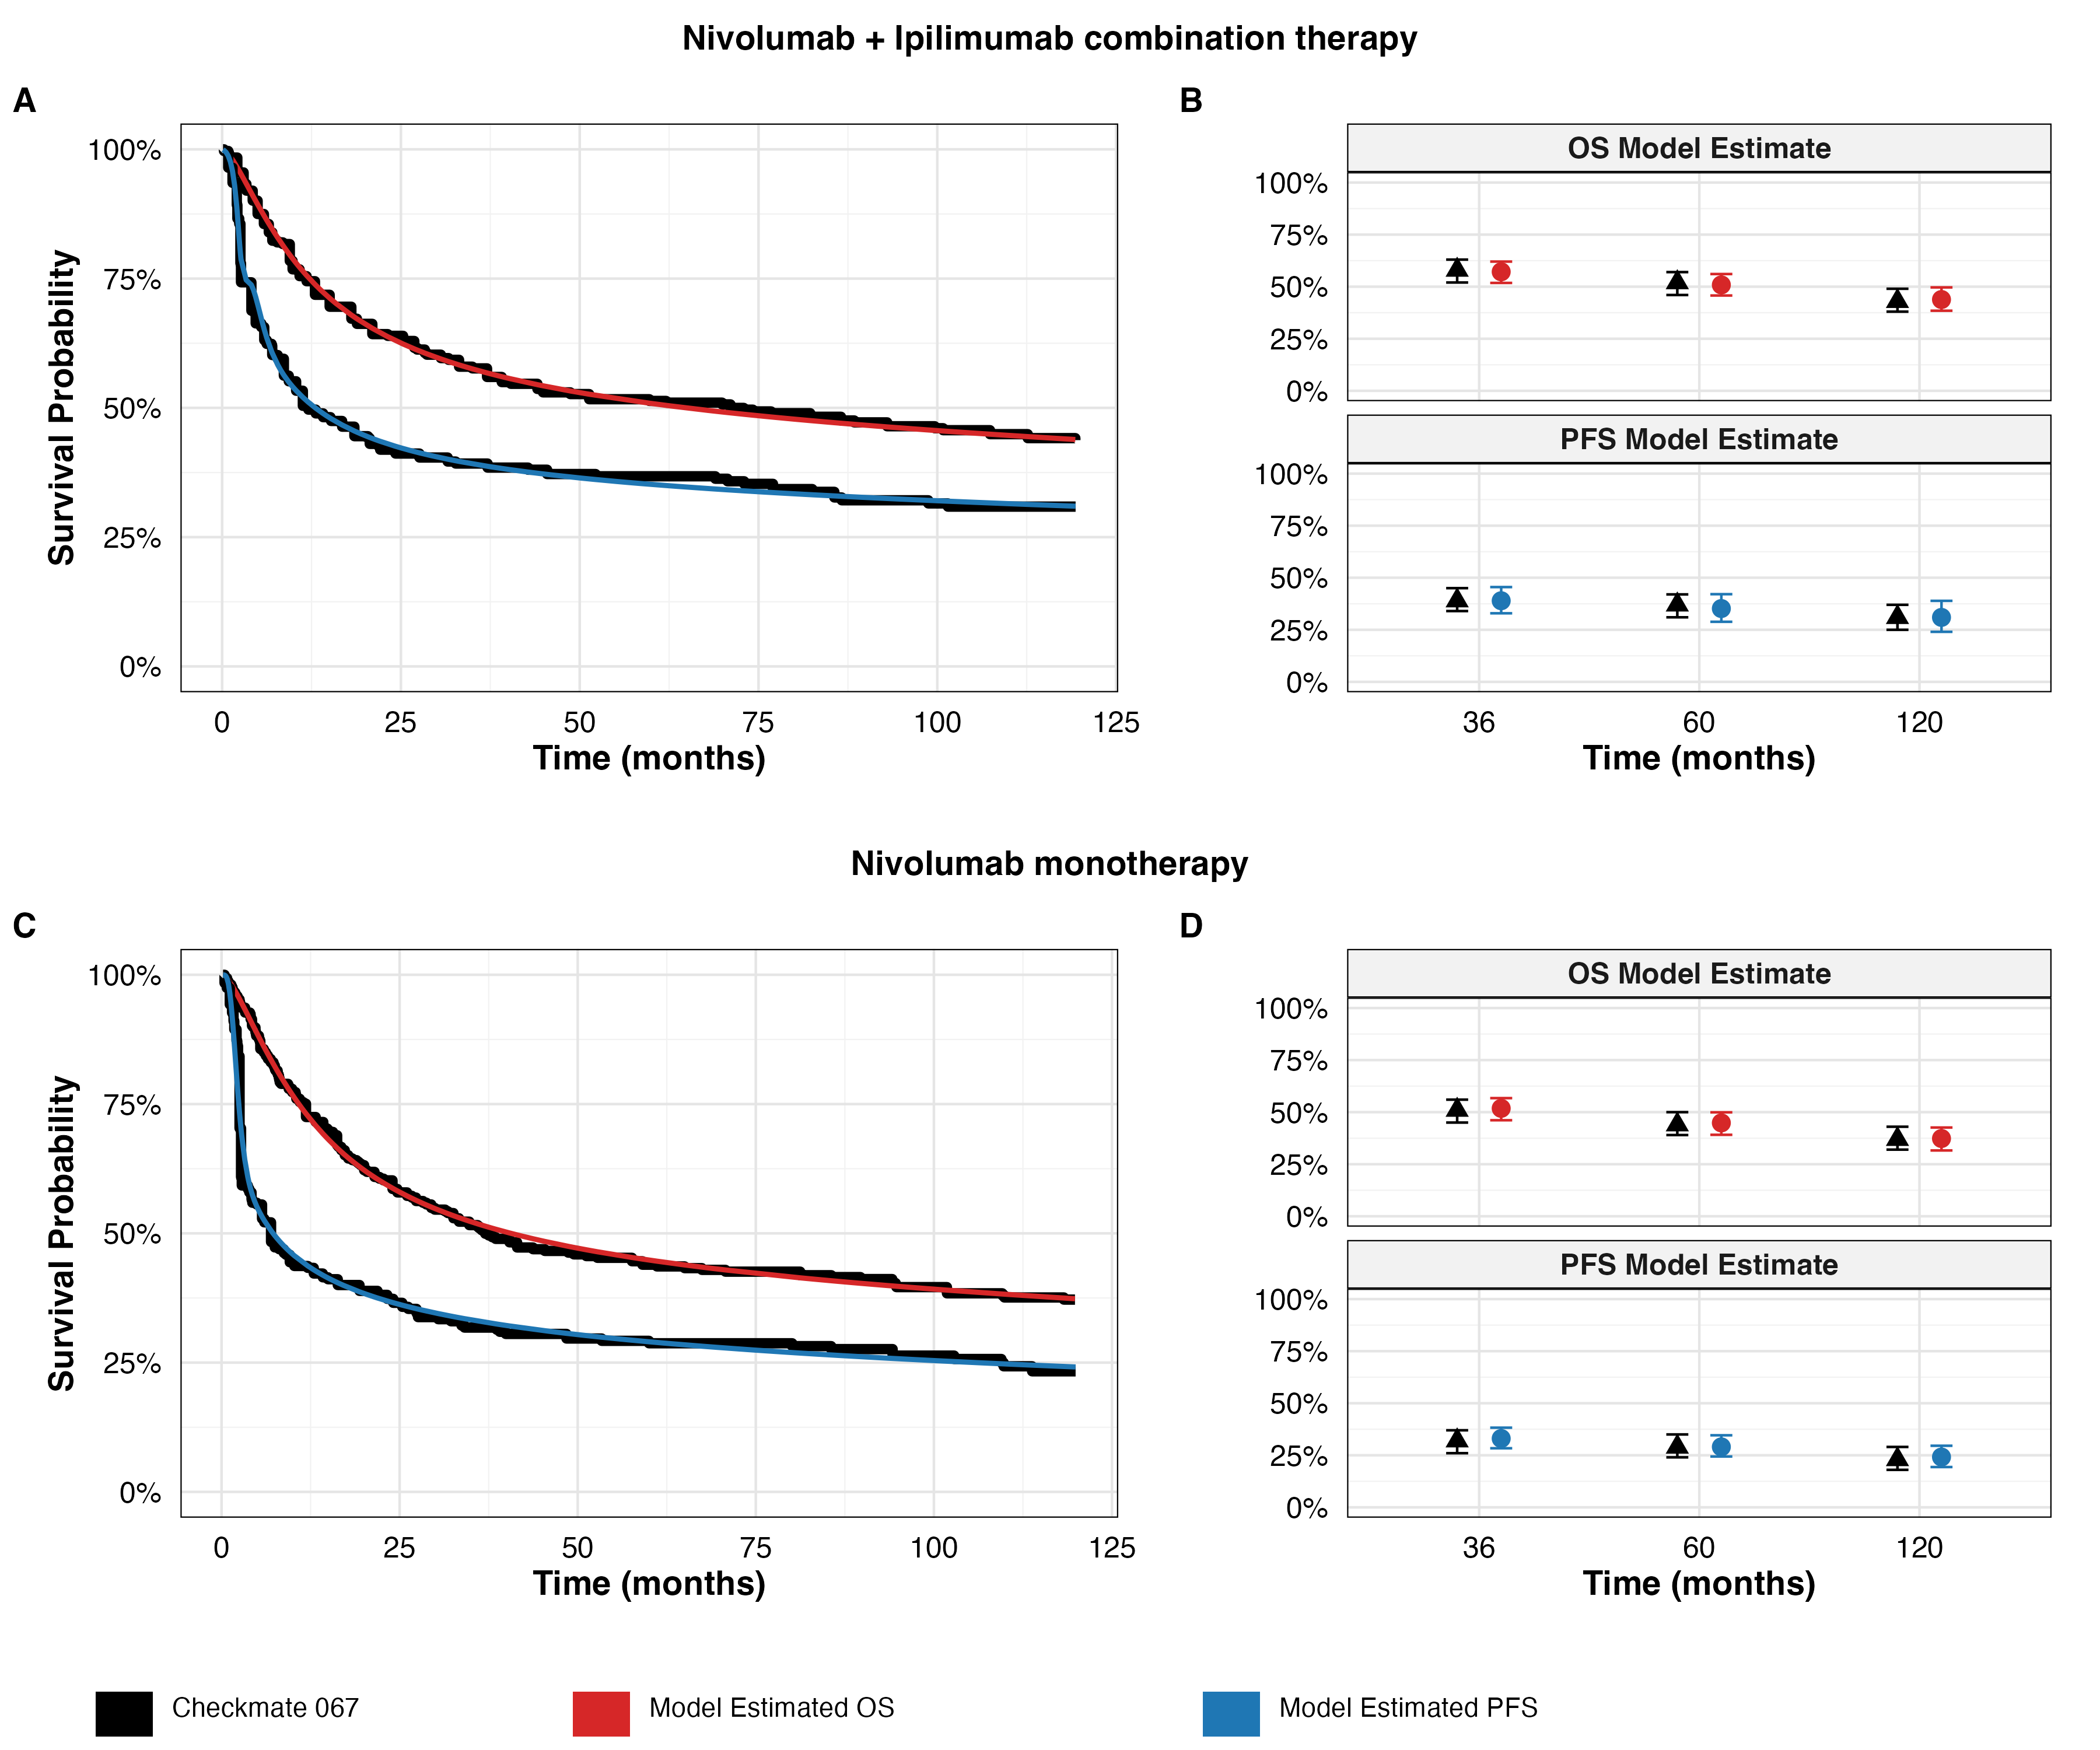
\includegraphics[width=0.9\textwidth]{../outputs/survival_curves.png}
\caption{Model validation. (A) and (C) display the reconstructed Kaplan–Meier curves overlaid with the predicted OS and PFS curves for the combination and nivolumab monotherapy arms, respectively. (B) and (D) compare model estimates at 30, 60, and 120 months with the published data. The smooth curves represent the model predictions, while the superimposed points with error bars denote published estimates and their confidence intervals.}
\label{fig:validation}
\end{figure}

\subsection{Biomarker-Based Strategy}\label{biomarker-based-strategy}

In addition to the standard treatment strategies, we simulated a
biomarker-driven approach. Based on the results of Tarantino et al.,
genomic heterogeneity and ploidy can predict intrinsic resistance to
PD-1 blockade with a reported positive predictive value (PPV) of 90\%,
sensitivity of 33\%, and specificity of 97\%. In our model, all patients
undergo a one-time genomic test (cost: \$5,000), and based on the test's
performance characteristics, patients are probabilistically assigned to
either:

\begin{itemize}
\item
  \textbf{Combination Therapy (nivolumab + ipilimumab)} if predicted
  resistant, or
\item
  \textbf{Nivolumab Monotherapy} if predicted sensitive.
\end{itemize}

This biomarker-based strategy is then compared with the standard,
non--biomarker-based approach.

\subsection{Counterfactual Survival
Estimates}\label{counterfactual-survival-estimates}

To further elucidate the heterogeneity in survival outcomes among
patients receiving single-agent anti--PD-1 therapy, we derived
counterfactual survival functions that delineate the extremes of patient
response. Our underlying hypothesis is that the overall survival (OS)
and progression-free survival (PFS) observed in the nivolumab
monotherapy arm represent a composite of two distinct subpopulations:
patients who respond favorably to anti--PD-1 therapy and those who are
intrinsically resistant. We assumed that the survival experience of
responders is upper-bounded by that observed under combination therapy
(Nivolumab + Ipilimumab), while the survival outcomes for intrinsically
resistant patients are markedly lower.

Mathematically, we express the monotherapy survival model function as a
weighted average:

\[
S_{\text{mon}} = w \times S_{\text{comb}} + (1 - w) \times S_{\text{resistant}},
\]

where \(S_{\text{mon}}\) is the survival probability in the nivolumab
monotherapy arm, \(S_{\text{comb}}\) represents the survival probability
for responders (assumed to match the combination therapy survival), and
\(S_{\text{resistant}}\) is the counterfactual survival probability for
intrinsically resistant patients. In our base-case analysis, we assumed
that 60\% of patients are responders (i.e., \(w = 0.6\)) and 40\% are
intrinsically resistant. An analogous procedure was applied to the PFS
curves. Counterfactual survival curves are presented in Figure
\hyperref[fig:counterfactual]{\ref{fig:counterfactual}}.

\begin{figure}[h]
\centering
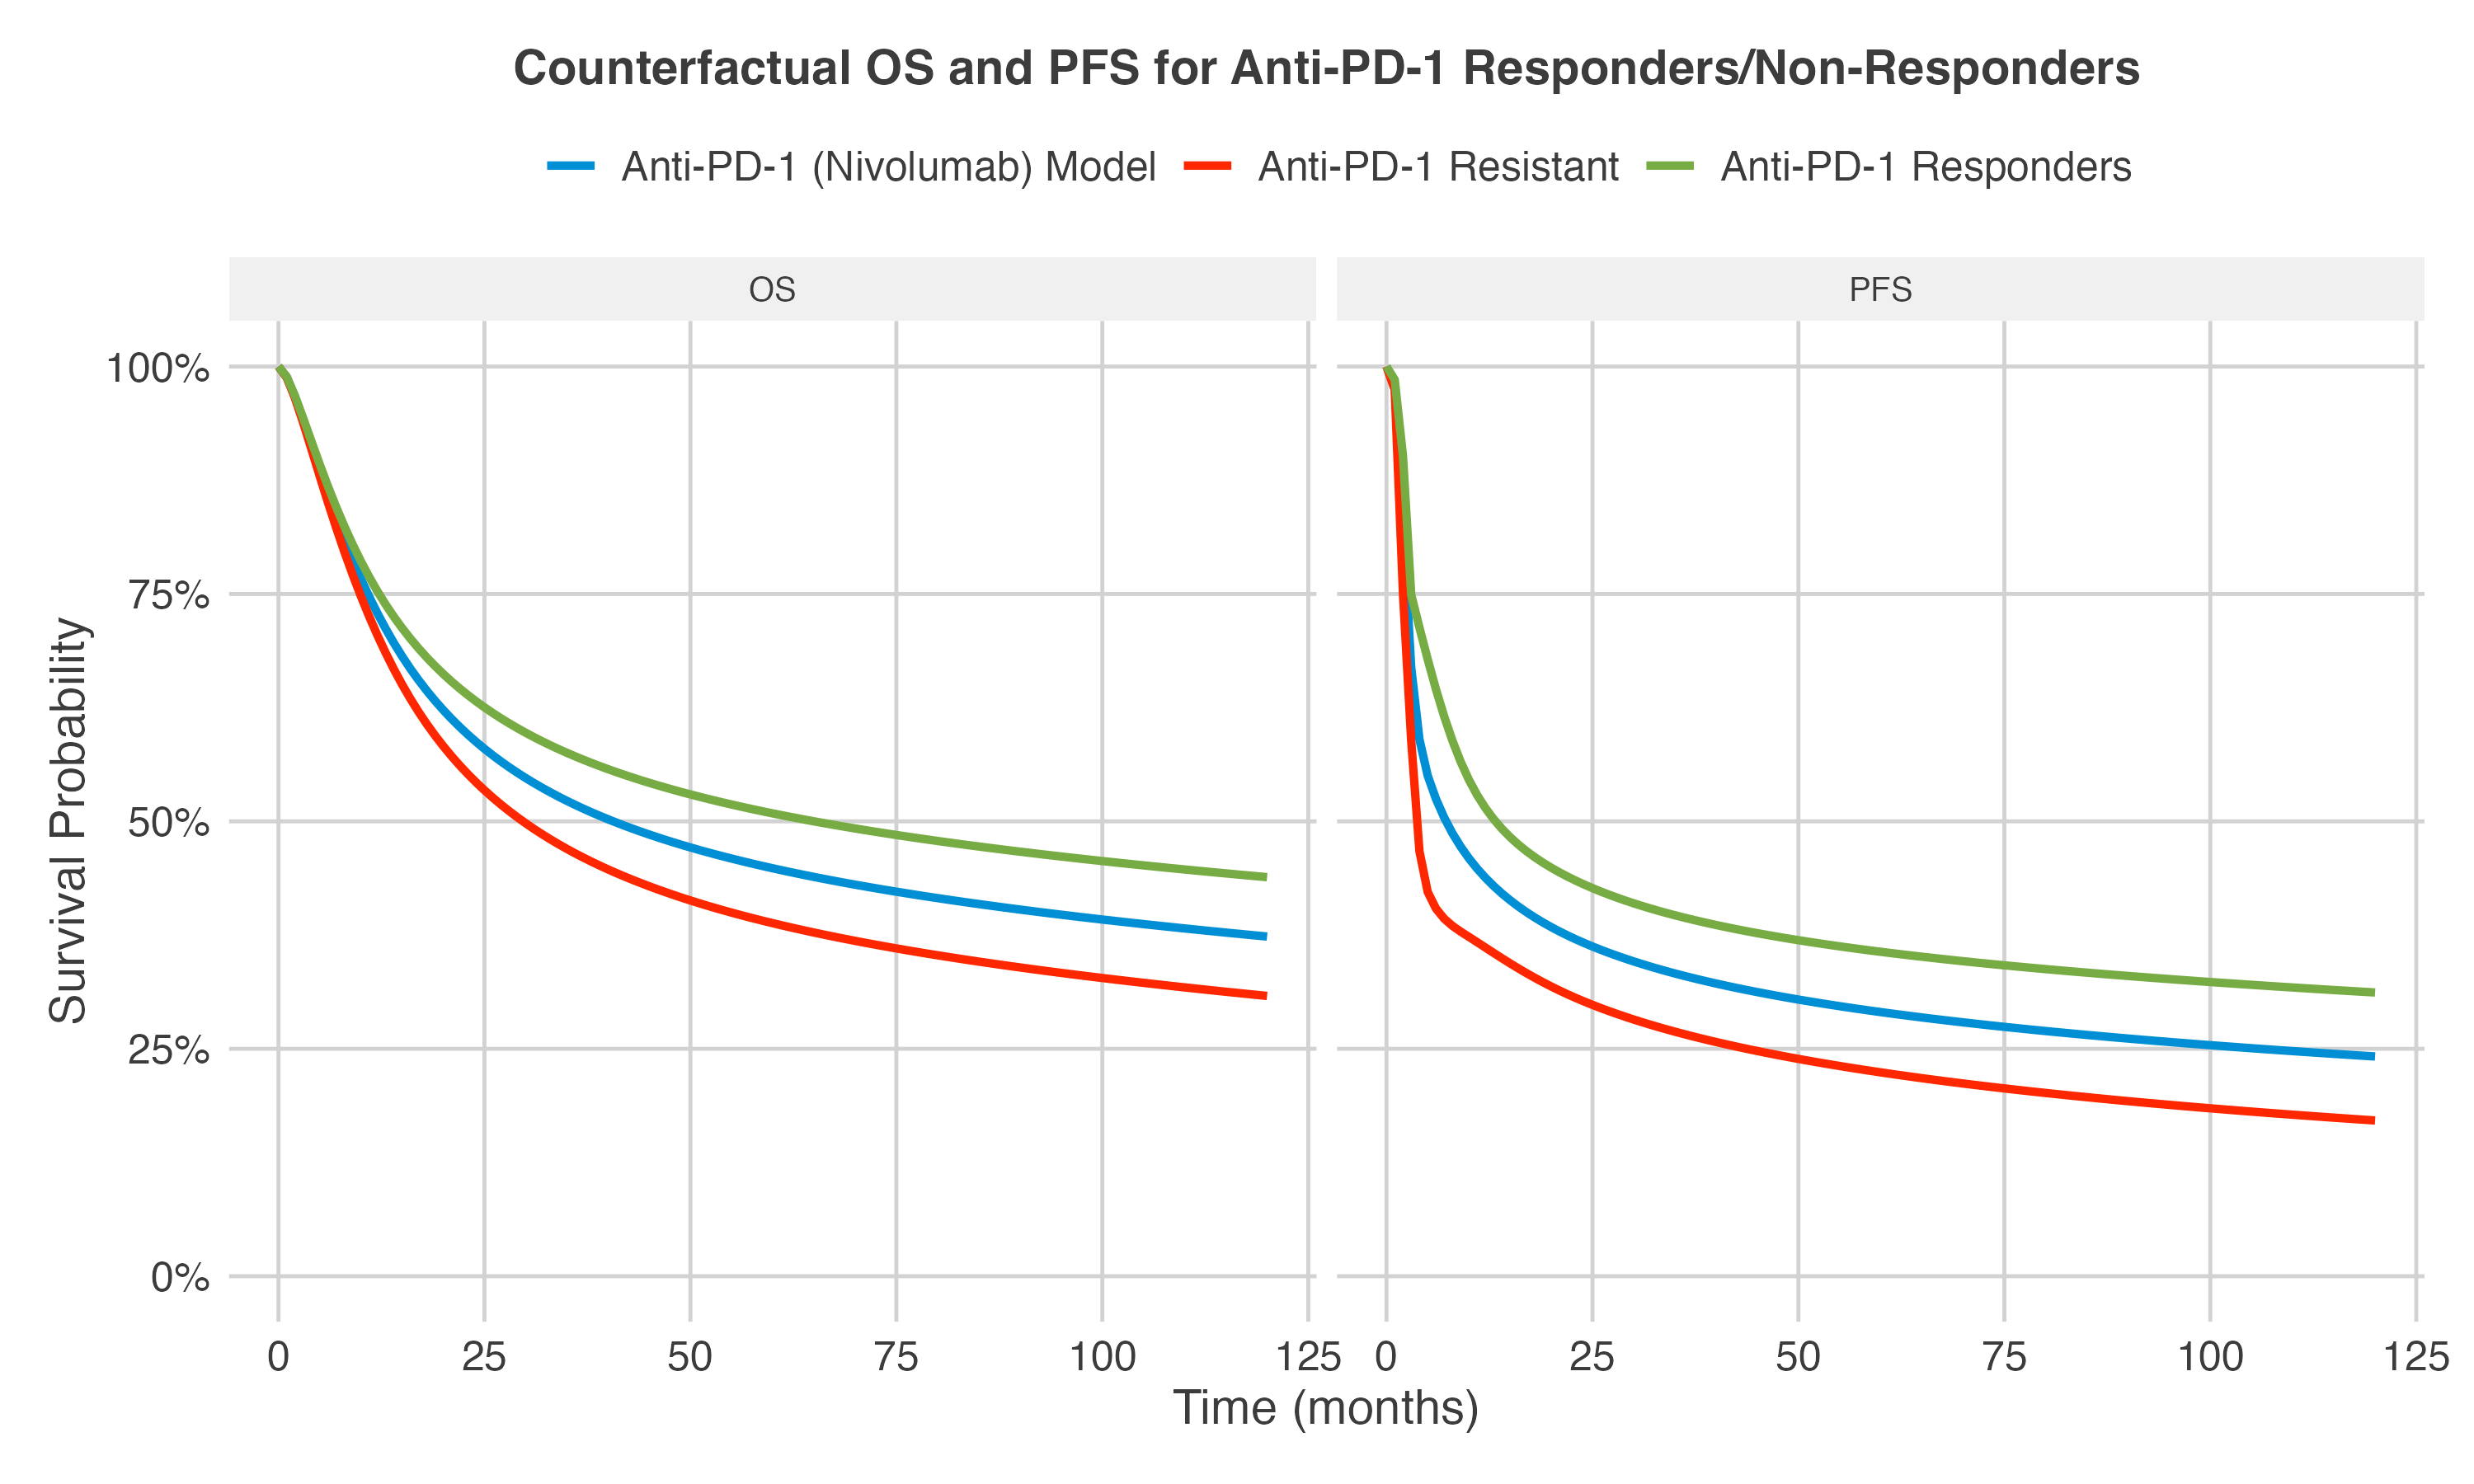
\includegraphics[width=0.9\textwidth]{../outputs/counterfactual_survival.png}
\caption{Counterfactual survival estimates. The solid lines represent the observed Kaplan–Meier curves for the nivolumab monotherapy arm, while the dashed lines denote the derived counterfactual survival functions for responders and intrinsically resistant patients.}
\label{fig:counterfactual}
\end{figure}

We generated predictions over a common time vector (0--120 months) from
our fitted survival models---namely. These predictions allowed us to
compute the counterfactual survival functions for the intrinsically
resistant and responsive subgroups. In effect, our approach provides
bounds on the survival outcomes under single-agent therapy: the
best-case scenario (for responders) is upper-bounded by the combination
therapy survival curve, while the worst-case scenario is represented by
the derived counterfactual for intrinsically resistant patients.

Furthermore, to assess the robustness of our findings, we incorporated
these counterfactual estimates into our probabilistic sensitivity
analysis. In this analysis, we varied the weighting parameter \(w\) as
well as the limits of the survival bounds to account for uncertainty in
the classification of responders versus non-responders. This sensitivity
analysis enables us to evaluate how deviations from our base-case
assumptions might influence the cost-effectiveness of a biomarker-based
treatment allocation strategy.

\subsection{Model Parameters}\label{model-parameters}

Table \hyperref[tab:parameters]{\ref{tab:parameters}} summarizes the key
model parameters, including survival probabilities, health utilities,
costs, and genomic test characteristics. To ensure the table fits within
the text width, we use the LaTeX \texttt{\textbackslash resizebox}
command.

\resizebox{\textwidth}{!}{
\begin{threeparttable}
\caption{Model Parameters}
\label{tab:parameters}
\begin{tabular}{@{}lll@{}}
\toprule
\textbf{Parameter} & \textbf{Value} & \textbf{Source / Comments} \\ \midrule
Cycle Length (months)        & 1                         & Assumed \\
Time Horizon (years)         & 10                        & Assumed \\
Utility\textsubscript{PF}     & 0.85                      & Literature/Assumption \\
Utility\textsubscript{PD}     & 0.65                      & Literature/Assumption \\
Cost\textsubscript{PF} (per cycle)  & \$1,000                & Assumed \\
Cost\textsubscript{PD} (per cycle)  & \$3,000                & Assumed \\
Cost of Genomic Test         & \$5,000                   & Tarantino et al. (adjusted) \\
Transition Prob. (Death) – Nivo Monotherapy  & 0.02 (monthly)          & Derived from CheckMate 067 calibration \\
Transition Prob. (Death) – Nivo+Ipi   & 0.015 (monthly)         & Derived from CheckMate 067 calibration \\
Transition Prob. (Progression) – Nivo Monotherapy  & 0.04 (monthly)          & Derived from CheckMate 067 calibration \\
Transition Prob. (Progression) – Nivo+Ipi   & 0.03 (monthly)         & Derived from CheckMate 067 calibration \\
Biomarker Sensitivity        & 33\%                     & Tarantino et al. \\
Biomarker Specificity        & 97\%                     & Tarantino et al. \\
Biomarker PPV                & 90\%                     & Tarantino et al. \\
Prevalence of Intrinsic Resistance & 20\%             & Assumed \\ \bottomrule
\end{tabular}
\begin{tablenotes}
\footnotesize
\item \textit{Note}: Transition probabilities were estimated by fitting parametric and spline models to the reconstructed IPD from the CheckMate 067 trial. Costs and utilities are based on published literature and expert opinion.
\end{tablenotes}
\end{threeparttable}
}

\subsection{Cost-Effectiveness
Analysis}\label{cost-effectiveness-analysis}

Using our calibrated Markov model, we simulated three treatment
strategies over a 10-year horizon:

\begin{enumerate}
\def\labelenumi{\arabic{enumi}.}
\item
  \textbf{Nivolumab Monotherapy}
\item
  \textbf{Combination Nivolumab + Ipilimumab}
\item
  \textbf{Biomarker-Based Strategy:} Patients first undergo genomic
  testing and are then assigned to combination therapy (if predicted
  resistant) or nivolumab monotherapy (if predicted sensitive).
\end{enumerate}

For each strategy, we calculated total costs, QALYs, and the incremental
cost-effectiveness ratio (ICER), applying a 3\% annual discount rate.
Deterministic one-way sensitivity analyses and probabilistic sensitivity
analyses (using Monte Carlo simulation with 100,000 iterations) were
performed to evaluate parameter uncertainty.

\section{Results}\label{results}

{[}Insert the calibrated model results here. For example, report the
simulated total costs, QALYs, and ICERs for each treatment strategy.
Provide details on the sensitivity analyses---both deterministic and
probabilistic---to illustrate the robustness of the findings.{]}

\section{Discussion}\label{discussion}

Our analysis indicates that both nivolumab monotherapy and combination
nivolumab plus ipilimumab yield favorable long-term survival outcomes
relative to historical controls. However, the higher toxicity and cost
associated with combination therapy underscore the need for a more
refined treatment allocation strategy. By incorporating genomic
predictors of intrinsic resistance, our biomarker-based strategy
potentially allocates combination therapy only to those patients most
likely to benefit, while sparing others from unnecessary toxicity and
cost.

The close alignment between our reconstructed Kaplan--Meier curves and
the published CheckMate 067 data supports the robustness of our survival
models. Furthermore, our sensitivity analyses suggest that even under
parameter uncertainty, the biomarker-driven strategy remains
cost-effective---assuming a willingness-to-pay threshold of \$100,000
per QALY.

Several limitations warrant discussion. First, our survival models are
extrapolated beyond the observed trial data, and long-term outcomes may
differ. Second, while the genomic test parameters are promising, they
require further prospective validation. Finally, our cost
inputs---derived from published literature and expert opinion---may not
capture all regional or temporal variations in treatment expenses.

Future research should integrate real-world data to further refine these
estimates and explore the inclusion of additional biomarkers and
treatment modalities. Nonetheless, our findings provide a strong
rationale for personalized treatment strategies in advanced melanoma,
with the potential to improve clinical outcomes and optimize resource
allocation.

\renewcommand\refname{References}
\bibliography{mybibfile.bib}


\end{document}
